\documentclass[a4paper,12pt]{article}


\usepackage[T1]{fontenc}
\usepackage[utf8]{inputenc}
\usepackage[frenchb]{babel}


\usepackage{graphicx}
\usepackage{xspace}


\title{Compte rendu de travaux pratiques\\ \small ou un meilleur titre}
\author{Vincent Denechaud, Olivier Maillet, Alice Odier, Félix Tora}
\date{Vendredi 24 janvier 2014}

\newcommand\ett{Everhart et Thornley\xspace}




\begin{document}

\maketitle

Voilà où on pourrait mettre l'introduction, sur les techniques MEB sans trop en faire.


\section{Les différentes sources électroniques du MEB}

Des électrons sont accélérés depuis la cathode vers l'échantillon que l'on souhaite étudier. Du fait de leur énergie cinétique, les électrons pénètrent dans la matière de l'échantillon en formant ce que l'on appelle une poire d'interaction (figure \ref{fig:poire_int}).

\begin{figure}
\centering
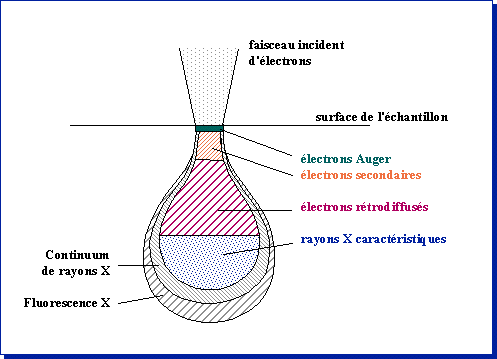
\includegraphics[width = 0.8 \textwidth]{images/poire_int.png}
\caption{Poire d'interaction : on distingue les différents type de rayonnements issus de l'interaction entre le faisceau électronique incident et l'échantillon.}
\label{fig:poire_int}
\end{figure}


En réponse à cette excitation, la matière revient à l'équilibre en émettant du rayonnement X ainsi que des électrons, 
de sorte que le cortège électronique des atomes composant l'échantillon possède une configuration d'équilibre énergétique. 
On peut classer les émissions électroniques selon différentes catégories.


Lorsque les électrons viennent interagir avec l'échantillon, ils sont, pour la plupart, rétrodiffusés de manière élastique.
Autrement dit, ces électrons interagissent avec les noyaux des atomes de l'échantillon de sorte à conserver leur énergie cinétique.
Ainsi, ces électrons ont une grande profondeur d'échappée et un grand libre parcours moyen dans l'échantillon.
De fait, ces électrons sont très sensibles à la composition chimique de l'échantillon, plus particulièrement, 
au numéro atomique Z des atomes constituant l'échantillon.
Les atomes les plus lourds (Z grand) vont ré-émettre plus d'électrons que les atomes plus légers. L'utilisation des électrons rétrodiffusés permet donc d'avoir un contraste chimique sur l'observation de l'échantillon.
Même s'ils ont une grande longueur de pénétration, ces électrons permettent une résolution spatiale (contraste topographique) de Xnm (figure \ref{fig:poire_int}).

En autre des électrons diffusés de manière quasi-élastique, une autre partie de ces derniers est diffusée de manière inélastique par l'échantillon.
Ce sont les électrons dits secondaires. 
Ces électrons cèdent donc très vite leur énergie cinétique et ont un faible libre parcours moyen ainsi qu'une faible profondeur de pénétration dans l'échantillon. 
Néanmoins, étant donné que ces derniers ressortent très vite de l'échantillon, la résolution spatiale obtenue 
après leur détection est bien meilleure (de l'ordre de $5$nm) que celle obtenue avec les électrons rétrodiffusés.
Les électrons secondaires seront donc très utiles pour réaliser un bon contraste topographique.
On notera cependant qu'il y a beaucoup moins d'électrons du type secondaire que rétrodiffusé. L'utilisation des électrons secondaires nécessite donc un temps de pose plus long pour réaliser un cliché.





\section{Echantillon éponge de Nickel}

L'observation de ce premier échantillon, une éponge de nickel, va nous permettre d'illustrer l'utilisation des différentes techniques présentées précédemment.

\subsection{Détecteur d'\ett}

Utilisant comme technique d'imagerie intiale les électrons secondaires receuillis par le détecteur d'\ett,
on accède à une première observation de l'échantillon présentée figure \ref{fig:ni_es}. Comme déjà évoqué,
cette technique a l'avantage d'offrir une grande profondeur de champ à l'image obtenue. Cette première
technique d'imagerie permet un contraste de profondeur de champ et donc de visualiser spatialement la forme
de l'échantillon.

\begin{figure}
\centering
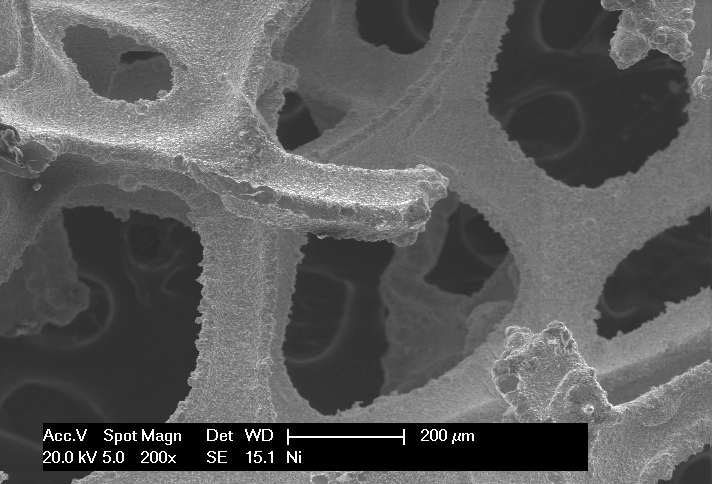
\includegraphics[width = 0.7 \textwidth]{images/ni_es.png}
\caption{Observation de l'éponge de nickel utilisant les électrons secondaires receuillis par le détecteur d'\ett. L'échantillon est ici grossi 200 fois.}
\label{fig:ni_es}
\end{figure}

Le détecteur d'\ett permet aussi de récolter des électrons rétrodiffusés. Ces électrons rétrodiffusés sont
collectés dans un angle solide bien précis, ainsi l'image obtenue à l'aide de cette technique présente une
certaine profondeur de champ mais aussi des effets d'ombre et de lumière. Ces effets sont dus à l'angle
d'incidence des électrons collectés. L'image obtenue à l'aide de cette technique est présentée figure
\ref{fig:ni_er_rasant}.

\begin{figure}
\centering
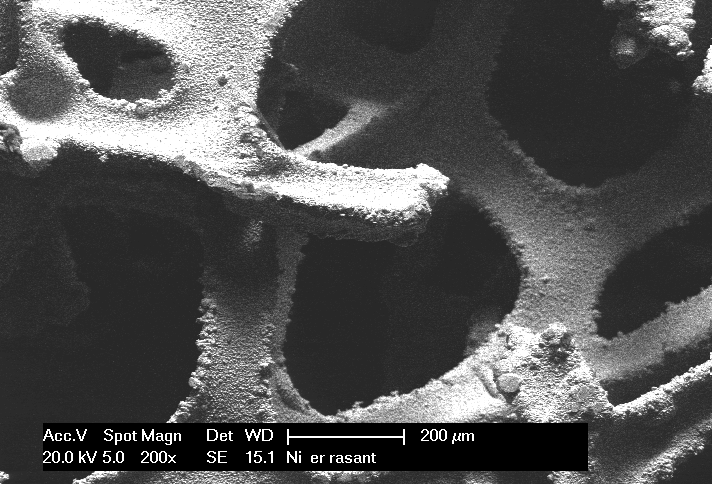
\includegraphics[width = 0.7 \textwidth]{images/ni_er_rasant.png}
\caption{Observation de l'éponge de nickel utilisant les électrons rétodiffuséss receuillis par le détecteur d'\ett. L'échantillon est ici grossi 200 fois.}
\label{fig:ni_er_rasant}
\end{figure}


\subsection{Détecteur à semi-conducteur}

L'utilisation du détecteur à semi-conducteur permet de collecter un grand nombre d'électrons rétrodiffusés
et d'obtenir deux types d'imagerie. L'utilisation du mode $A+B$ permet d'obtenir une image avec un contraste
en composition chimique. L'image de l'éponge de nickel obtenue avec cette technique est présentée à la figure
\ref{fig:ni_er_apb}. Sur cette image on voit que la profondeur de champ du cliché est très faible. Cependant
le contraste en composition chimique permet d'obtenir d'autres informations tout aussi importantes.

On peut voir sur l'échantillon certaines excroissances qui apparaissent plus foncées. Cette image permet d'observer
la présence d'mpuretées sur le matériau, tout du moins de parties faites d'éléments différents.


\begin{figure}
\centering
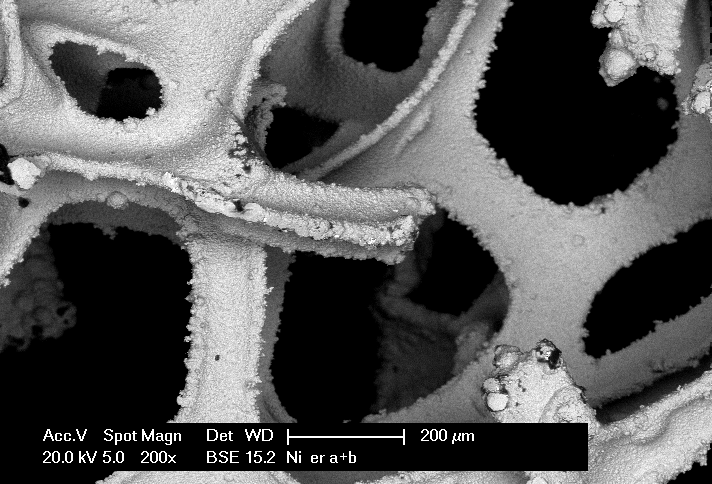
\includegraphics[width = 0.7 \textwidth]{images/ni_er_apb.png}
\caption{Observation de l'éponge de nickel utilisant les électrons rétodiffuséss receuillis par le détecteur à semi-conducteur en mode $A+B$. L'échantillon est ici grossi 200 fois.}
\label{fig:ni_er_apb}
\end{figure}



Le détecteur à semi-conducteur permet également de réaliser un cliché différent en utilisant les mêmes électrons
rétrodiffusés. L'image réalisée avec le mode $A-B$ est présentée sur la figure \ref{fig:ni_er_amb}. Sur ce cliché
le contraste est topographique.

\begin{figure}
\centering
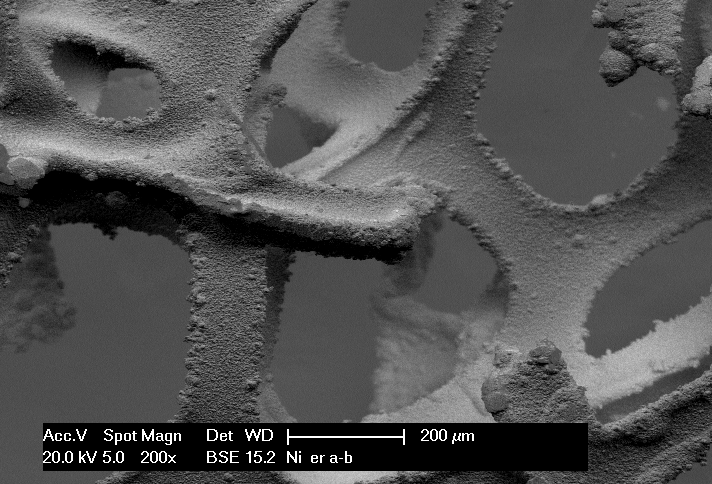
\includegraphics[width = 0.7 \textwidth]{images/ni_er_amb.png}
\caption{Observation de l'éponge de nickel utilisant les électrons rétodiffuséss receuillis par le détecteur à semi-conducteur en mode $A-B$. L'échantillon est ici grossi 200 fois.}
\label{fig:ni_er_amb}
\end{figure}
 

\section{Echantillon de silicium}

L'étude, avec les techniques d'imagerie du microscope électronique à balayage, d'un échantillon de silicium permet d'obtenir un grand nombre d'informations.

\subsection{Structure cristallographique de l'échantillon}

On réalise une image de l'échantillon de silicium en collectant les électrons secondaires avec le détecteur d'\ett.
Le cliché obtenu est présenté sur la figure \ref{fig:si_es}. On garde à l'esprit qu'il présente un contraste topographique.
On observe des structures pyramidales en bas-relief ou en haut-relief. Les conditions d'éclairage du cliché ne permettent
pas d'opter pour l'une ou l'autre des solutions (bas-relief ou haut-relief). Ces structures nous informent sur la structure
du matériau et l'observation de ce cliché nous permet de penser que la structure de l'échantillon est cristalline.



\begin{figure}
\centering
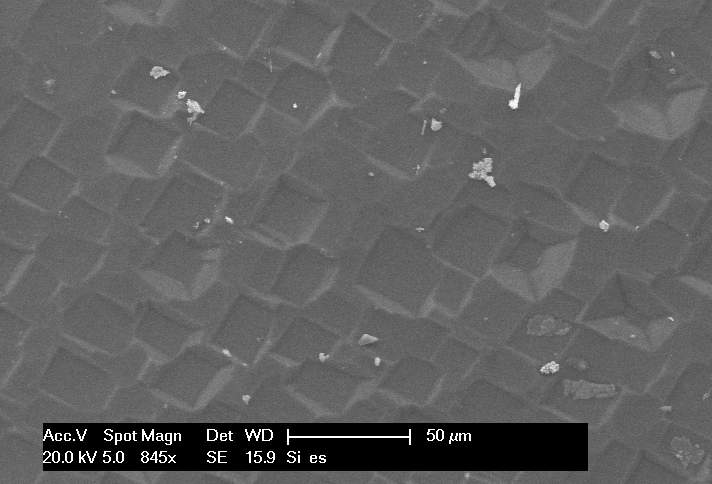
\includegraphics[width=0.7\textwidth]{images/si_es.png}
\caption{Observation d'un échantillon de silicium utilisant les électrons secondaires collectés dans le détecteur d'\ett. L'échantillon est ici grossi 845 fois.}
\label{fig:si_es}
\end{figure}

Afin de déterminer si les pyramides sont en bas-relief ou non on utilise un autre cliché. La figure \ref{fig:si_er_rasant} présente
un cliché réalisé à l'aide du détecteur de \ett mais en colelctant les électrons rétrodiffusés. Les électrons utilisés étant rasants,
on observe des effets d'ombre et de lumière. Par exemple une poussière en haut à droite du cliché projette son ombre vers le bas.
On en déduit que l'éclairage provient du haut du cliché. Ainsi il est maintenant possible de se prononcer sur l'enfoncement des pyramides.
Les faces éclairées sont celles situées en bas, ce qui veut dire que les pyramides sont en bas-relief.

\begin{figure}
\centering
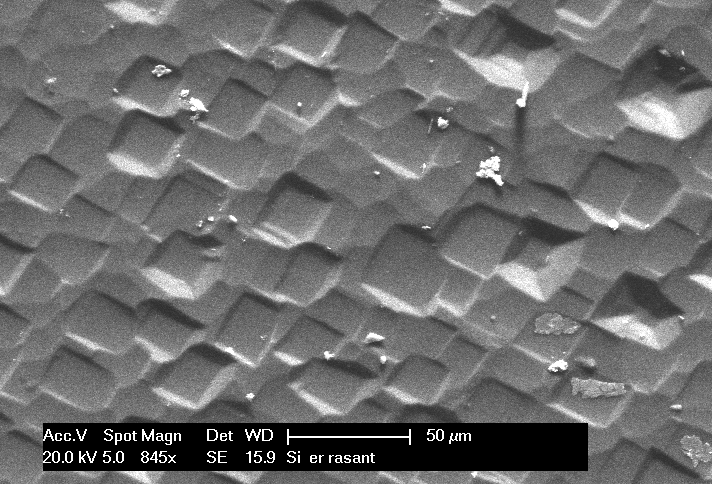
\includegraphics[width=0.7\textwidth]{images/si_er_rasant.png}
\caption{Observation d'un échantillon de silicium utilisant les électrons rétrodiffusés collectés dans le détecteur d'\ett. L'échantillon est ici grossi 845 fois.}
\label{fig:si_er_rasant}
\end{figure}


\section*{Conclusion}

Et puis tout à la fin on pourrait mettre une petite conclusion aux petits oignons.


\end{document}
